%%%%%%%%%%%%%%%%%%%%%%%%%%%%%%%%%%%%%%%%%
% Simple Sectioned Essay Template
% LaTeX Template
%
% This template has been downloaded from:
% http://www.latextemplates.com
%
% Note:
% The \lipsum[#] commands throughout this template generate dummy text
% to fill the template out. These commands should all be removed when 
% writing essay content.
%
%%%%%%%%%%%%%%%%%%%%%%%%%%%%%%%%%%%%%%%%%

%----------------------------------------------------------------------------------------
%	PACKAGES AND OTHER DOCUMENT CONFIGURATIONS
%----------------------------------------------------------------------------------------

\documentclass[12pt]{article} % Default font size is 12pt, it can be changed here

\usepackage{hyperref}


\usepackage{geometry} % Required to change the page size to A4
\geometry{a4paper} % Set the page size to be A4 as opposed to the default US Letter

\usepackage{graphicx} % Required for including pictures
\graphicspath{{Images/}}

\usepackage{cite}


\usepackage{float} % Allows putting an [H] in \begin{figure} to specify the exact location of the figure

\linespread{1.2} % Line spacing

%\setlength\parindent{0pt} % Uncomment to remove all indentation from paragraphs

%\graphicspath{{Images/}} % Specifies the directory where pictures are stored

\begin{document}

%----------------------------------------------------------------------------------------
%	TITLE PAGE
%----------------------------------------------------------------------------------------

\begin{titlepage}

\newcommand{\HRule}{\rule{\linewidth}{0.5mm}} % Defines a new command for the horizontal lines, change thickness here

\center % Center everything on the page

\textsc{\LARGE University of Potsdam}\\[1.5cm] % Name of your university/college
\textsc{\Large Declarative Modeling}\\[0.5cm] % Major heading such as course name
%\textsc{\large Timetabling Project}\\[0.5cm] % Minor heading such as course title

\HRule \\[0.4cm]
{ \huge \bfseries Timetabling Project}\\[0.4cm] % Title of your document
\HRule \\[1.5cm]

\begin{minipage}{0.4\textwidth}
\begin{flushleft} \large
\emph{Author:}\\
  Robert Sch\"afer \\
  Felix Kubicek
\end{flushleft}
\end{minipage}
~
\begin{minipage}{0.4\textwidth}
\begin{flushright} \large
\emph{Supervisor:} \\
  Javier Romero Davila
\end{flushright}
\end{minipage}\\[4cm]

{\large \today}\\[3cm] % Date, change the \today to a set date if you want to be precise


%\includegraphics{Logo}\\[1cm] % Include a department/university logo - this will require the graphicx package

\vfill % Fill the rest of the page with whitespace

\end{titlepage}

%----------------------------------------------------------------------------------------
%	TABLE OF CONTENTS
%----------------------------------------------------------------------------------------

\tableofcontents % Include a table of contents

\newpage % Begins the essay on a new page instead of on the same page as the table of contents 

%----------------------------------------------------------------------------------------
%	INTRODUCTION
%----------------------------------------------------------------------------------------

\section{Introduction} 

In the course of this project we developed a planning tool to support the timtabeling process, performed each semester, at the Institute of Computer Science.
For this purpose we developed a web application that can be used for generating timetables for university courses, presenting the timetables, etc.
Besides Answer Set Programming (ASP) \cite{ASP} was used to develop specific rules that must or should be considered for the planning process, as well as for finding approriate timetables. 
The following sections will give a short overview of our general approach to the problem, as well as the architecture of our planning system.


\section{User Centered Desing} 





\section{Architecture} % Sub-section

\subsection{Data Model} 

\begin{figure}[h]
    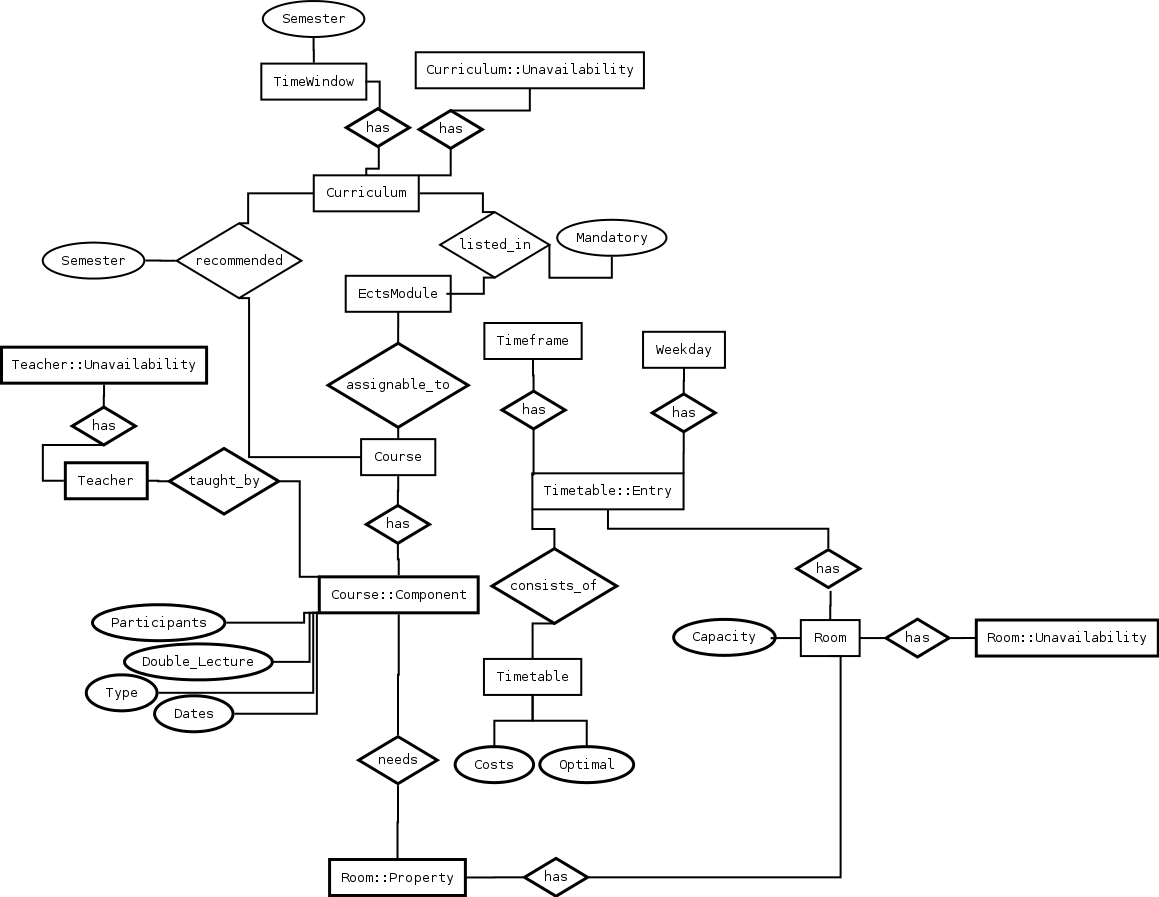
\includegraphics[width=\textwidth]{TimetablingER_Dia.png}
    \caption{Database schema, modeled as entity-relationship diagram \cite{Chen76}.}
    \label{fig:schema}    
\end{figure}

Figure~\ref{fig:schema} demonstrates the database schema.
A timetable, which consists of several timetable entries, represents a complete schedule.
Timetables have costs, resulting from penalty values of the ASP soft constraints.
The timetables with the lowest costs are optimal solutions.
A timetable entry is an assignment of a certain component of a course, e.g. a lecture, to a certain room, as well as to a specific weekday and timeframe. 
Course Components, taught by a specific teacher, have got a certain type, e.g lecture, tutorial, etc.
Besides course components can have multiple dates, participants and several room properties.
If, for instance, the course component has to take place in a computer pool then the room assigned to the course component has to be declared as computer pool through a certain property.
The courses are linked to a specific curricular through modules.
Besides a course can be recommended for a semester in a certain curricular.
The advantage over recommending modules for a specific semester is that courses with different recommendations can now be assigned to the same module.
The modules listed in a specific curricular can be elective or mandatory.
A curricular can be assigned to multiple time windows.
The concept of time windows was introduced to allow students participating the \emph{Informatik Lehramt Bachelor} program to study with little overlapping of courses.
In order to prevent overlapping, mandatory lectures for student teachers must be assigned to a determined set of time windows dependent on the semester recommendation.
Finally there are unavailabilities for teachers, curricular and rooms.
All unavailabilities are linked to a specific day and time-slot which is not shown in the diagram for clarity reasons.

\section{Conclusion}


%----------------------------------------------------------------------------------------
%	BIBLIOGRAPHY
%----------------------------------------------------------------------------------------
\bibliographystyle{plain}
\bibliography{report}


%----------------------------------------------------------------------------------------

\end{document}